\documentclass[11pt,a4paper]{article}

% Packages
\usepackage[utf8]{inputenc}
\usepackage[T1]{fontenc}
\usepackage{lmodern}
\usepackage[english,bahasai]{babel}
\usepackage[a4paper,margin=2.5cm]{geometry}
\usepackage{setspace}
\usepackage{graphicx}
\usepackage{booktabs}
\usepackage{tabularx}
\usepackage{longtable}
\usepackage{float}
\usepackage{caption}
\usepackage[autostyle=false,style=english]{csquotes}
\usepackage[style=apa,backend=biber]{biblatex}
\DeclareLanguageMapping{bahasai}{english-apa}
\usepackage{tikz}
\usetikzlibrary{positioning,arrows.meta}
\usepackage[hidelinks]{hyperref}

\addbibresource{../references.bib}
\graphicspath{{figures/}}
\setstretch{1.15}
\captionsetup{font=small,labelfont=bf}

% Report Info
\newcommand{\judul}{PowerShift: Paket Pensiun Dini PLTU dan PLTS Atap untuk Transisi Energi Sistem Jawa-Bali}
\newcommand{\sumber}[1]{\par\smallskip{\footnotesize Sumber: #1}}

\begin{document}

\pagenumbering{gobble}
\begin{titlepage}
\centering
\vspace*{0.5cm}
{\Large\bfseries LAPORAN PROYEK MINOR\par}
\vspace{0.4cm}
{\large MK4066 Perubahan Iklim (Layanan)\par}
\vspace{0.8cm}
{\LARGE\bfseries \judul\par}
\vspace{0.8cm}
{\large Topik 13: Transisi Energi, PLTS Atap dan Pensiun Dini PLTU\par}
\vspace{0.7cm}

\includegraphics[width=3.2cm]{logo_itb}\par
\vspace{0.7cm}
{\large Kelompok 17\par}
\vspace{0.4cm}
{\footnotesize
\begin{tabular}{l l @{\hspace{1.2cm}} l l}
10124084 & Azzahra Rizqi Saffa & 15024052 & Alzena Atha Audya \\
10524012 & Danica Giovanni & 15024071 & Lidya Savarani Tarigan \\
10524057 & Nayma Feby Nur Safitri & 15124027 & Jessica Aulia Cahyana \\
10623042 & Pande I Made Niko Mevano W P & 15124032 & Qabil Radhiqa Handoyo \\
12023096 & Dimas Rayhan & 15124066 & Angga Setiawan \\
12225128 & Franzeska Jessica Mattea & 15325014 & Elja Manuella Joesta Damanik \\
12324059 & Fahri Masis Nurhidayat & 15325021 & Muhammad Rafi Hikaru Rahman \\
13123086 & Ananda Ghibran Fadlilah & 15325093 & Alya Gita Khairani \\
13123129 & Muhammad Azhar Shiddiq & 15524057 & Haidar Islama Muhammad Firdaus \\
13224028 & Isnaya Zalfa Kamila & 18023017 & Raynee Soe Putra \\
13424036 & Magdalena Conny H.C.L.T & 18124013 & Kayla Olivia Putri \\
13523144 & Muhamad Nazih Najmudin & 18224076 & Bram Sebastian Pangaribuan \\
\end{tabular}

}
\vfill
{\large Institut Teknologi Bandung\par}
{\large 2026\par}
\end{titlepage}


\pagenumbering{roman}
\tableofcontents
\clearpage
\pagenumbering{arabic}

\section{Latar dan Isu}
\label{sec:latar}

\subsection{Sektor Ketenagalistrikan dan Komitmen Iklim}

Pemanasan global akibat aktivitas manusia telah meningkatkan risiko cuaca ekstrem, kekeringan, dan kenaikan muka laut \parencite{P-IPCC-2023}. Di Indonesia, pembangkit listrik tenaga uap (PLTU) batu bara adalah sumber emisi dan polusi udara yang dominan. Sistem Jawa-Madura-Bali (Jamali), interkoneksi terbesar di Indonesia, saat ini mengoperasikan 57 unit PLTU terhubung jaringan PLN dengan kapasitas 30,8 GW dan emisi sekitar 169 juta ton CO$_2$ per tahun \parencite{D-GEM-GCPT}.

Pemerintah sudah memiliki dasar hukum untuk mengakhiri PLTU lebih awal. Perpres 112/2022 mengamanatkan peta jalan pengakhiran operasi PLTU \parencite{R-PERPRES-112-2022}, dan Permen ESDM 10/2025 menurunkannya menjadi tujuh kriteria pensiun dini serta kewajiban kajian PLN paling lama enam bulan \parencite{R-PERMEN-ESDM-10-2025,B-CNN-20250422}. Di sisi energi bersih, PLTS atap adalah teknologi yang paling cepat dipasang oleh masyarakat. Namun hingga Juli 2025 kapasitas terpasangnya baru 538 MWp di 10.882 pelanggan \parencite{B-KONTAN-ROOFTOP-2025}.

\subsection{Rantai Hambatan Transisi}

Kajian ini berangkat dari pengamatan bahwa hambatan utama transisi bukan ketidaktertarikan warga terhadap PLTS atap, melainkan posisi keuangan PLN dan negara. Rantainya digambarkan pada Gambar~\ref{fig:rantai}.

\begin{figure}[H]
\centering
\begin{tikzpicture}[node distance=0.55cm, box/.style={draw, rounded corners, align=center, font=\footnotesize, text width=3.4cm, minimum height=1.1cm, fill=gray!6}, arr/.style={-{Stealth}, thick}]
\node[box] (a) {Oversupply Jamali dan kontrak take-or-pay PLTU IPP};
\node[box, right=of a] (b) {PLTS atap mengurangi penjualan PLN, biaya kapasitas PLTU tetap dibayar};
\node[box, right=of b] (c) {Kerugian PLN menjadi beban APBN karena tarif ditetapkan pemerintah};
\node[box, below=of c] (d) {Permen ESDM 2/2024: net metering dihapus, kuota PLTS atap};
\node[box, left=of d] (e) {PLTS atap tidak menarik bagi rumah tangga};
\node[box, left=of e] (f) {Pensiun dini dianggap mahal: Cirebon-1 batal (2025), beralih ke phase down};
\draw[arr] (a) -- (b); \draw[arr] (b) -- (c); \draw[arr] (c) -- (d); \draw[arr] (d) -- (e); \draw[arr] (e) -- (f);
\end{tikzpicture}
\caption{Rantai hambatan transisi PLTS atap dan pensiun dini PLTU}
\label{fig:rantai}
\sumber{disusun dari \textcite{B-TENGGARA-2024}, \textcite{P-IEEFA-2017}, dan \textcite{B-PETROMINDO-CIREBON-BATAL}}
\end{figure}

PLN membayar pembayaran kapasitas kepada pembangkit swasta (IPP) selama unit tersedia, terlepas dari listriknya dipakai atau tidak \parencite{P-IEEFA-2017}. Ketika listrik di Jawa-Bali berlebih, PLN menolak membayar penuh ekspor PLTS atap karena akan menaikkan biaya pokok penyediaan (BPP) yang ujungnya dibebankan ke subsidi \parencite{B-TENGGARA-2024}. Revisi aturan PLTS atap lewat Permen ESDM 2/2024 kemudian menghapus net metering dan menetapkan kuota per wilayah \parencite{R-PERMEN-ESDM-2-2024,B-TENGGARA-2024}. Di sisi PLTU, rencana pensiun dini Cirebon-1 yang didukung Asian Development Bank (ADB) dibatalkan pada Desember 2025. PLN menilai percepatan lima tahun memicu kewajiban kompensasi sekitar Rp60 triliun dan beralih ke pendekatan phase down, yaitu memensiunkan PLTU di akhir kontrak \parencite{B-PETROMINDO-CIREBON-BATAL,B-MONGABAY-202601}.

Hambatan ini juga dikenal dalam literatur. Pensiun dini sebelum aset habis disusutkan menimbulkan aset terdampar \parencite{P-KEFFORD-2018}, sedangkan ruang fiskal dan akses pendanaan internasional Indonesia terbatas \parencite{P-RESOSUDARMO-2023}.

\subsection{Pertanyaan Kajian}

Kajian ini menjawab tiga pertanyaan proyek minor dengan fokus pada sistem Jawa-Bali dan Cirebon-1 sebagai kasus utama:
\begin{enumerate}
  \item Dampak apa yang ditimbulkan PLTU Jawa-Bali, dan siapa yang menanggungnya?
  \item Apakah PLTS atap, pensiun dini, atau gabungan keduanya layak dari sisi PLN dan negara?
  \item Inovasi apa yang dapat membantu pemerintah menyusun paket yang dapat diterima PLN?
\end{enumerate}
Tiga hipotesis diuji dengan model PowerShift (Bagian~\ref{sec:inovasi}). H1: PLTS atap tanpa pensiun PLTU memperburuk neraca PLN. H2: memasangkan PLTS atap dengan pensiun dini memperkecil kerugian itu bila kompensasi didanai pihak luar. H3: ada kombinasi kebijakan yang membuat neraca PLN mendekati netral.

\section{Dampak}
\label{sec:dampak}

\subsection{Sebaran dan Emisi PLTU Sistem Jawa-Bali}

Gambar~\ref{fig:peta} dan Tabel~\ref{tab:pltu} memperlihatkan 57 unit PLTU operasi yang terhubung jaringan PLN di Jawa-Bali. PLTU captive milik industri tidak dimasukkan karena berada di luar jaringan PLN. Sebanyak 18,8 GW dimiliki IPP dan 12,0 GW dimiliki PLN. Banten dan Jawa Tengah menampung lebih dari dua pertiga kapasitas.

\begin{figure}[H]
\centering
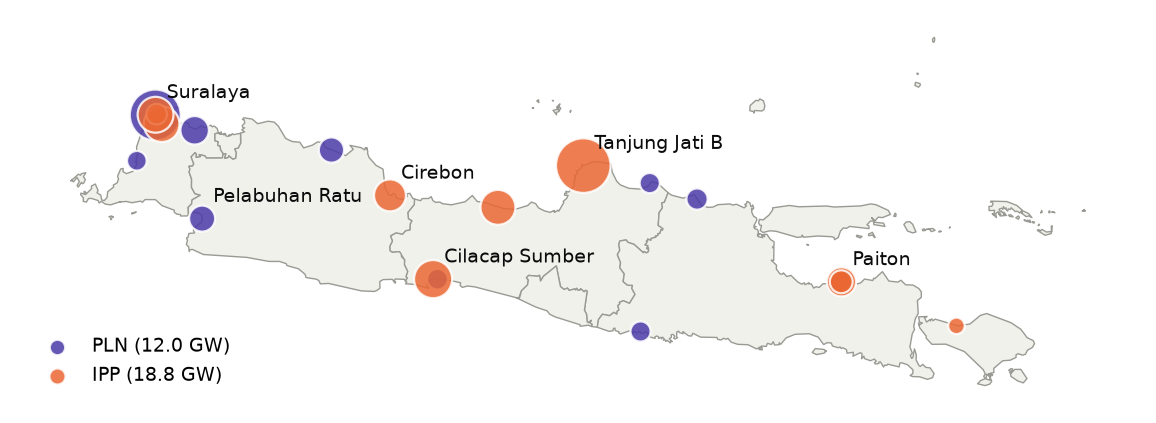
\includegraphics[width=\textwidth]{peta_pltu}
\caption{PLTU terhubung jaringan PLN di Jawa-Bali menurut pemilik (ukuran lingkaran sebanding kapasitas)}
\label{fig:peta}
\sumber{\textcite{D-GEM-GCPT}, batas wilayah \textcite{D-GEOBOUND}, diolah kelompok}
\end{figure}

\begin{table}[H]
\centering
\caption{PLTU jaringan PLN Jawa-Bali per provinsi}
\label{tab:pltu}
\small
\begin{tabular}{lrrrrrr}
\toprule
Provinsi & Unit & MW & IPP (MW) & PLN (MW) & Mt CO$_2$/tahun & Kematian/tahun \\
\midrule
Banten & 19 & 10.527 & 4.642 & 5.885 & 57,6 & 2.722 \\
Jawa Tengah & 15 & 10.090 & 8.800 & 1.290 & 52,4 & 2.610 \\
Jawa Timur & 12 & 6.155 & 3.365 & 2.790 & 36,3 & 1.592 \\
Jawa Barat & 8 & 3.624 & 1.584 & 2.040 & 19,9 & 1.676 \\
Bali & 3 & 426 & 426 & 0 & 2,7 & 110 \\
\midrule
Total & 57 & 30.822 & 18.817 & 12.005 & 168,9 & 8.710 \\
\bottomrule
\end{tabular}

\sumber{\textcite{D-GEM-GCPT} untuk kapasitas dan emisi. Kematian dini dihitung dari faktor rata-rata armada \textcite{P-CREA-IESR-2023}, kecuali Cirebon-1 yang memakai angka khusus CREA}
\end{table}

\subsection{Dampak Kesehatan}

CREA dan IESR memodelkan bahwa emisi PLTU batu bara pada 2022 menyebabkan sekitar 10.500 kematian dini dan biaya kesehatan US\$7,4 miliar \parencite{P-CREA-IESR-2023}. Jawa Barat adalah provinsi paling terdampak dengan lebih dari 4.000 kematian per tahun, disusul Banten (2.000) dan Jawa Tengah (1.700). Temuan ini sejalan dengan studi regional yang memproyeksikan kenaikan beban penyakit akibat ekspansi PLTU di Asia Tenggara \parencite{P-KOPLITZ-2017}.

Dampak tidak merata antar-PLTU. Di wilayah Jawa-Bali-Sumatra, CREA menempatkan Muara Karang, Lontar, Cirebon, Cirebon-2, dan Cilacap sebagai pembangkit dengan biaya kesehatan per kWh tertinggi karena dekat permukiman padat \parencite{P-CREA-IESR-2023}. Untuk Cirebon-1, CREA memperkirakan pensiun pada 2035 menghindari 6.370 kematian dan US\$4,4 miliar biaya kesehatan selama 2036-2042 \parencite{B-ECOBUSINESS-CIREBON}. Artinya, nilai kesehatan dari pensiun dini sangat bergantung pada PLTU mana yang dipilih.

\subsection{Pekerja dan Daerah}

Cirebon-1 mempekerjakan sekitar 300 orang, dan hanya 50 di antaranya berasal dari desa sekitar. CELIOS memperkirakan sedikitnya 14.000 pekerja terdampak bila Cirebon-1 dan Pelabuhan Ratu dipensiunkan, termasuk pekerja tidak langsung \parencite{B-ECOBUSINESS-CIREBON}. Sebaliknya, PLTS atap termasuk teknologi energi yang paling padat karya, sekitar 24,72 job-year per MW \parencite{P-CEEW-2017}. Transisi yang adil membutuhkan program alih keterampilan agar pekerja PLTU dapat berpindah ke sektor ini.

\subsection{Beban Rumah Tangga dan Fiskal}

Penjualan listrik PLN pada 2025 mencapai 317,69 TWh, dan 133,41 TWh di antaranya untuk rumah tangga \parencite{B-CNBC-SALES-2025}. Jawa-Bali menyerap 220,8 TWh atau 69,5\% dari penjualan nasional, dengan Jawa Barat sebagai pasar terbesar (63,5 TWh) \parencite{D-PLN-STAT-2025}. Subsidi listrik 2026 diusulkan Rp97,37-104,97 triliun untuk 44,88 juta pelanggan, dengan BPP Rp1.828-1.920 per kWh \parencite{B-KONTAN-SUBSIDI-2026}. Pelanggan 450 VA dan 900 VA bersubsidi membayar Rp415 dan Rp605 per kWh, sedangkan rumah tangga 1.300-2.200 VA membayar Rp1.444,70 per kWh \parencite{B-KOMPASTV-TARIF-2026}. Karena tarif ditetapkan di bawah BPP, setiap perubahan biaya PLN pada akhirnya berpindah ke APBN.

Tanpa net metering, PLTS atap rumah tangga menjadi kurang menarik karena konsumsi rumah tangga tinggi pada malam hari. IESR memperkirakan adopsi PLTS atap akan lebih banyak terjadi di sektor komersial dan industri \parencite{B-PVMAG-QUOTA,P-IESR-PERMEN2}.

\subsection{Dampak pada Keandalan Sistem}

Pada Februari 2024 daya mampu pasok sistem Jamali tercatat 37.364 MW dengan beban puncak tertinggi 28.077 MW \parencite{B-MATAHARI-2024}. Statistik PLN 2025 mencatat kapasitas terpasang Jawa 52.575 MW dan daya mampu 49.681 MW, termasuk pembangkit sewa dan IPP \parencite{D-PLN-STAT-2025}. Selisih ini terjadi karena daya mampu pasok hanya menghitung pembangkit yang siap dioperasikan, sehingga kajian ini memakai angka cadangan dari PLN UIP2B dan MKI. White Paper Masyarakat Ketenagalistrikan Indonesia (MKI) memperkirakan reserve margin turun dari 37,5\% pada 2025 ke bawah rentang aman 33-35\% pada 2027 jika beban tumbuh 4,45\% per tahun tanpa tambahan pembangkit yang cukup \parencite{B-PETROMINDO-RESERVE}. Kondisi ini penting: selama listrik berlebih, satu PLTU dapat dipensiunkan tanpa diganti, tetapi setelah jendela itu menutup, setiap PLTU yang pensiun membutuhkan pembangkit pengganti.

\section{Opsi Respons}
\label{sec:opsi}

Empat opsi mitigasi dibandingkan dengan simulasi PowerShift (cara kerja di Bagian~\ref{sec:inovasi}). Seluruh angka keuangan adalah selisih kumulatif 2026-2040 terhadap baseline phase down, yaitu PLTU pensiun di akhir PPA atau umur desain dan PLTS atap tumbuh mengikuti tren dengan aturan sekarang. Hasilnya diringkas pada Tabel~\ref{tab:preset} dan Gambar~\ref{fig:preset}.

\begin{table}[H]
\centering
\caption{Hasil simulasi empat opsi, kumulatif 2026-2040 terhadap baseline phase down}
\label{tab:preset}
\small
\resizebox{\textwidth}{!}{\begin{tabular}{lrrrr}
\toprule
Indikator & PLTS atap saja & Pensiun dini saja & Paket Cirebon-1 & Paket seimbang \\
\midrule
Neraca PLN (Rp T) & -120,0 & 2,1 & -117,8 & 1,4 \\
Neraca negara, PLN + APBN (Rp T) & -132,6 & 2,1 & -130,5 & 3,5 \\
Dana luar ETM/JETP (Rp T) & 0,0 & 3,1 & 3,1 & 14,7 \\
Hemat tagihan pelanggan (Rp T) & 162,3 & 0,0 & 162,3 & 21,6 \\
CO$_2$ dihindari (Mt) & 158,3 & -0,9 & 157,5 & 21,4 \\
Kematian dini dihindari & 7.473 & 4.436 & 11.909 & 8.921 \\
Nilai kesehatan (Rp T) & 86,9 & 51,6 & 138,5 & 103,7 \\
PLTS atap 2040 (GWp) & 19,1 & 4,0 & 19,1 & 5,5 \\
Pembangkit pengganti (MW) & 0 & 660 & 660 & 2.580 \\
Kenaikan BPP maks. (Rp/kWh) & 37,0 & 0,0 & 36,1 & 3,0 \\
\bottomrule
\end{tabular}
}
\sumber{simulasi PowerShift, parameter pada Lampiran~\ref{app:asumsi}}
\end{table}

\subsection{Phase Down di Akhir PPA}

Opsi ini adalah kebijakan yang berjalan sekarang dan menjadi baseline. Kelebihannya, tidak ada biaya kompensasi dan risiko hukum terhadap kontrak IPP. Keterbatasannya, sebagian besar PLTU Jawa-Bali baru pensiun setelah 2040, sehingga emisi dan dampak kesehatan sekitar 8.700 kematian per tahun (Tabel~\ref{tab:pltu}) terus berlangsung.

\subsection{Penetrasi PLTS Atap}

Opsi ini mengembalikan nilai ekspor PLTS atap ke 65\%, menaikkan kuota Jawa-Bali menjadi 1.500 MW per tahun, mewajibkan 100 MW per tahun di gedung pemerintah, dan mengalihkan 5\% subsidi listrik untuk PLTS atap pelanggan 450/900 VA. Kapasitas PLTS atap pada 2040 naik dari 4,0 menjadi 19,1 GWp, menghindari 158 juta ton CO$_2$ dan sekitar 7.500 kematian dini. Keterbatasannya, neraca PLN memburuk sekitar Rp120 triliun karena pendapatan ritel berpindah ke pemilik PLTS atap, dan BPP naik hingga 37,0 Rp/kWh. Hasil ini mengonfirmasi H1 dan menjelaskan mengapa PLN menahan PLTS atap.

\subsection{Pensiun Dini PLTU}

Opsi ini memensiunkan Cirebon-1 pada 2035, sesuai kesepakatan dengan ADB \parencite{B-ADB-CIREBON}, dengan 75\% kompensasi dari dana luar. Kelebihannya, PLN berhenti membayar kapasitas IPP sehingga neracanya membaik Rp2,1 triliun, dan sekitar 4.400 kematian dini dihindari. Keterbatasannya, karena jendela oversupply sudah tertutup pada 2035, PLN tetap membutuhkan 660 MW pembangkit pengganti. Emisi juga praktis tidak turun karena energi Cirebon-1 dipasok PLTU lain.

\subsection{Paket Berpasangan}

Opsi ini menggabungkan kedua opsi sebelumnya (Paket Cirebon-1). Neraca PLN membaik sekitar Rp2,2 triliun dibanding PLTS atap saja, sehingga H2 terbukti, tetapi perbaikannya kecil dibanding kerugian dari pendapatan ritel. Manfaat kesehatannya paling besar, sekitar 11.900 kematian dini dihindari atau setara Rp138,5 triliun.

\subsection{Perbandingan Opsi}

\begin{figure}[H]
\centering
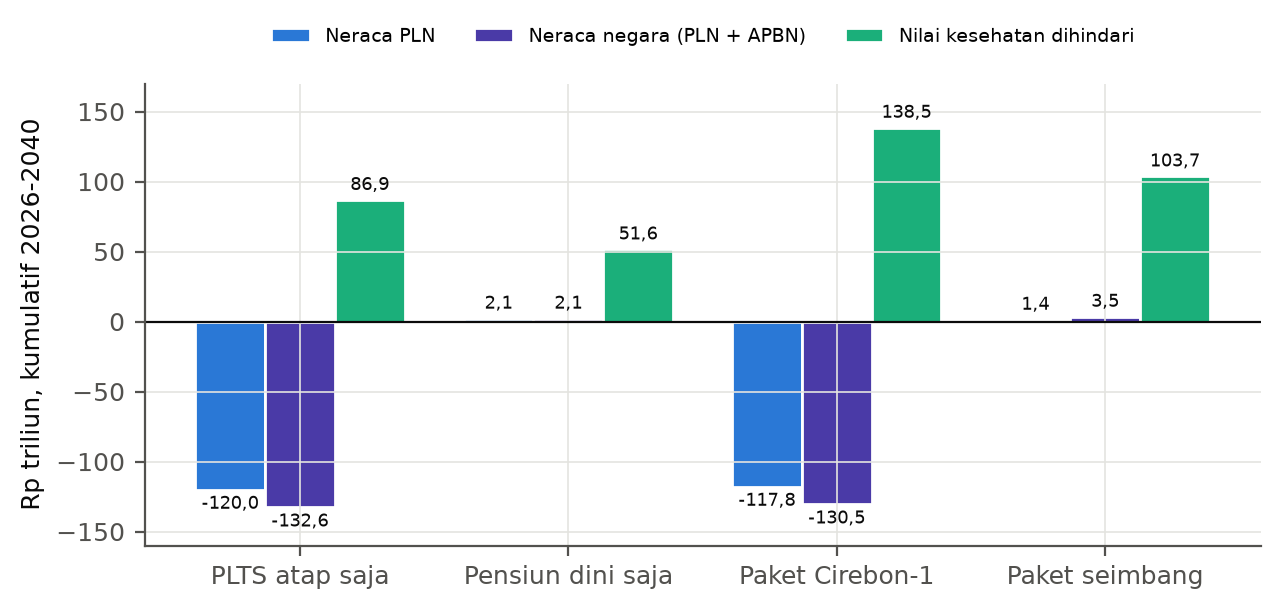
\includegraphics[width=\textwidth]{neraca_preset}
\caption{Neraca PLN, neraca negara, dan nilai kesehatan per opsi (kumulatif 2026-2040)}
\label{fig:preset}
\sumber{simulasi PowerShift}
\end{figure}

Gambar~\ref{fig:preset} menunjukkan pola yang konsisten: setiap opsi yang menambah PLTS atap secara besar membebani PLN dan APBN, sementara nilai kesehatannya berpindah ke masyarakat. Pensiun dini IPP dengan dana luar menguntungkan PLN, tetapi manfaat emisinya baru muncul bila energinya digantikan energi bersih. Karena itu dibutuhkan alat untuk mencari kombinasi yang seimbang, yang dijelaskan pada bagian berikut.

\section{Inovasi}
\label{sec:inovasi}

PowerShift adalah alat bantu keputusan berbasis web untuk merancang paket ``pensiun dini PLTU + PLTS atap'' di sistem Jawa-Bali. Alat ini menghitung siapa menanggung apa, yaitu PLN, APBN, dana luar, pelanggan, pekerja, dan warga di sekitar PLTU, setiap tahun dari 2026 sampai 2040. Gambar~\ref{fig:app} memperlihatkan tampilan utamanya.

\begin{figure}[H]
\centering
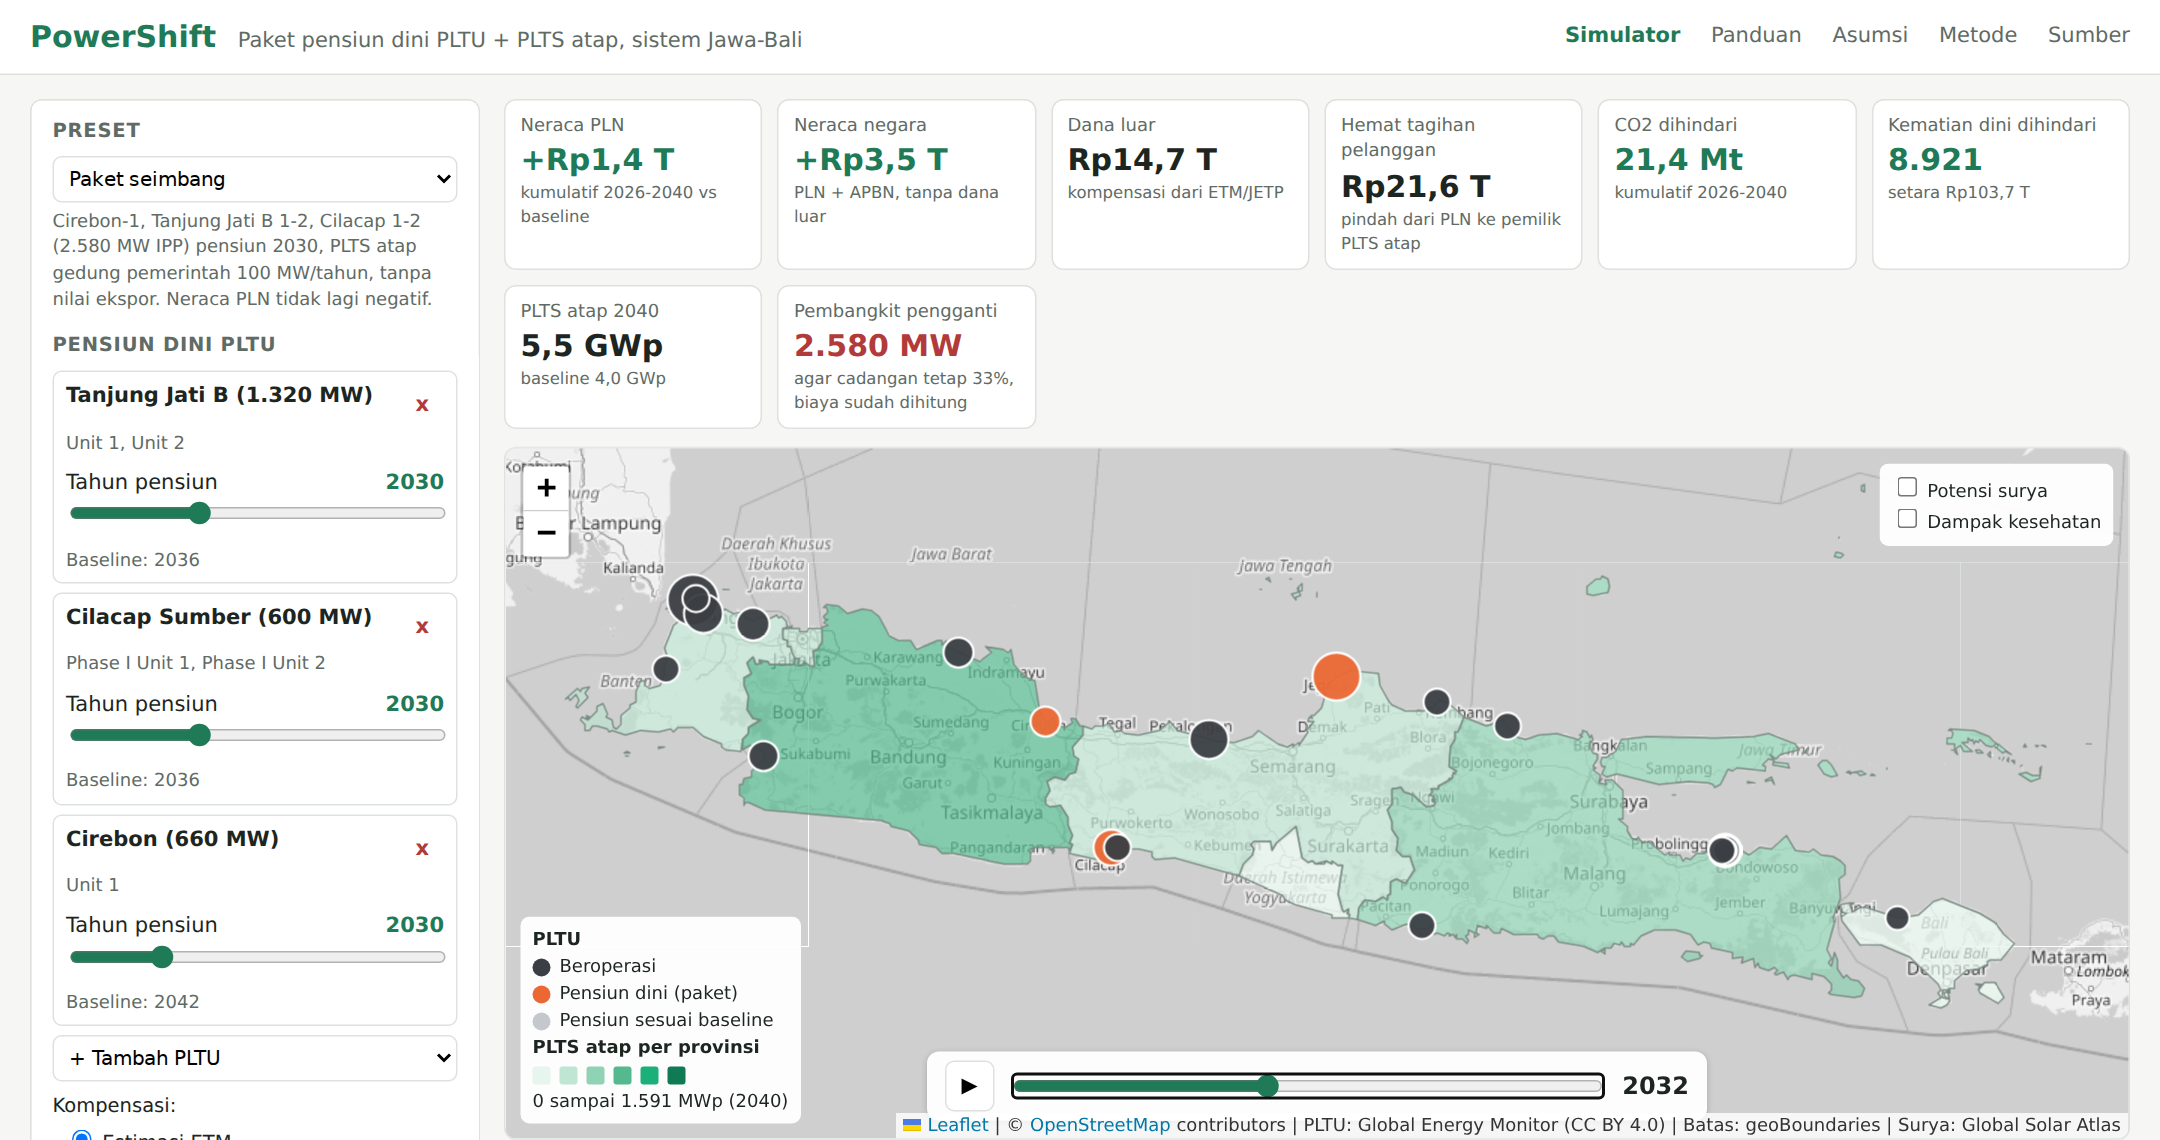
\includegraphics[width=\textwidth]{app_powershift}
\caption{Tampilan PowerShift untuk Paket seimbang pada tahun 2032. PLTU yang dipensiunkan dini berwarna jingga, warna provinsi menunjukkan kapasitas PLTS atap}
\label{fig:app}
\sumber{PowerShift, peta dasar OpenStreetMap contributors}
\end{figure}

\subsection{Kebaruan}

Alat yang sudah ada menjawab sebagian pertanyaan secara terpisah (Tabel~\ref{tab:kebaruan}). Belum ditemukan alat yang menghitung paket berpasangan PLTS atap terdistribusi dan pensiun PLTU per unit dari sisi neraca PLN dan APBN, padahal di titik inilah kebijakan selama ini macet.

\begin{table}[H]
\centering
\caption{PowerShift dibanding alat yang sudah ada}
\label{tab:kebaruan}
\small
\begin{tabularx}{\textwidth}{p{0.2\textwidth} X X}
\toprule
Alat & Yang dilakukan & Yang belum dilakukan \\
\midrule
Indonesia Energy Policy Simulator & Simulasi kebijakan nasional dan emisi \parencite{P-WRI-EPS} & Agregat nasional, tidak per PLTU dan tidak menghitung neraca PLN \\
TZ-CAT & Data per unit PLTU, biaya pengganti EBT skala besar \parencite{D-TZCAT,P-TZ-CONUNDRUM} & Lembar kerja untuk ahli, data 2022, tidak memuat PLTS atap \\
Kajian CREA dan IESR & Peringkat PLTU menurut biaya kesehatan \parencite{P-CREA-IESR-2023} & Laporan statis, tidak interaktif \\
SolarHub & Kalkulator PLTS atap per bangunan \parencite{P-SOLARHUB} & Tidak melihat dampak ke sistem dan PLN \\
En-ROADS & Simulator iklim global \parencite{P-ENROADS} & Tidak spesifik Indonesia \\
\midrule
PowerShift & Paket per unit PLTU dan PLTS atap, neraca PLN, APBN, dana luar, keandalan, kesehatan, kriteria Permen ESDM 10/2025, peta Jawa-Bali & Bukan model dispatch per jam \\
\bottomrule
\end{tabularx}
\sumber{penelusuran kelompok, November 2026}
\end{table}

\subsection{Cara Kerja}

Pengguna memilih PLTU dan tahun pensiunnya, nilai ekspor PLTS atap, kuota, PLTS atap gedung pemerintah, porsi subsidi yang dialihkan, sumber dana kompensasi, serta asumsi kompensasi (estimasi skema ETM atau klaim PLN). Model tahunan kemudian menghitung:
\begin{enumerate}
  \item \textbf{Adopsi PLTS atap.} Balik modal per segmen dihitung dari potensi surya per kabupaten \parencite{D-GSA-PVOUT}, tarif, dan porsi pemakaian sendiri. Perubahan adopsi mengikuti kurva pangsa pasar terhadap balik modal yang dipakai NREL \parencite{P-NREL-SOLARDS}, dibatasi kuota.
  \item \textbf{Neraca PLN.} Pendapatan yang hilang dan kompensasi ekspor dikurangkan, lalu ditambah biaya bahan bakar yang dihemat \parencite{B-KONTAN-DMO-2026}, pembayaran kapasitas IPP yang tidak lagi dibayar, dan dikurangi porsi kompensasi pensiun serta biaya pembangkit pengganti.
  \item \textbf{Neraca APBN dan negara.} Selisih PLN ditutup APBN, ditambah subsidi yang dihemat, tagihan gedung pemerintah yang dihemat, investasi PLTS pemerintah, dan porsi kompensasi APBN.
  \item \textbf{Keandalan.} Reserve margin dihitung dari data PLN dan MKI \parencite{B-MATAHARI-2024,B-PETROMINDO-RESERVE}. Mulai 2029 baseline dijaga di 33\%, sehingga PLTU yang pensiun dini harus diganti.
  \item \textbf{Dampak dan kriteria.} Emisi per unit dari GEM, kematian dini dari CREA, pekerja per MW, dan penilaian indikatif tujuh kriteria Pasal 11 Permen ESDM 10/2025.
\end{enumerate}

Hasil tampil sebagai kartu angka, peta PLTU dengan slider tahun 2026-2040, peta warna PLTS atap per provinsi, grafik neraca, dan tabel kriteria. Skenario dapat dibagikan lewat tautan, grafik serta data dapat diunduh, dan halaman Panduan menjelaskan setiap langkah penggunaan dengan tangkapan layar. PowerShift berupa situs statis (HTML, JavaScript, Leaflet, Chart.js) tanpa server sehingga dapat dihosting gratis \parencite{S-LEAFLET,S-CHARTJS}. Model diverifikasi dengan hitung tangan independen untuk Paket Cirebon-1 (Lampiran~\ref{app:hitung}) dengan selisih di bawah 0,01\%.

\subsection{Kecocokan untuk Indonesia}

PowerShift dibangun dari struktur yang khas Indonesia: PLN sebagai pembeli tunggal, kontrak take-or-pay IPP, harga batu bara DMO US\$70 per ton, subsidi 450/900 VA, oversupply Jawa-Bali yang akan habis, dan kriteria Permen ESDM 10/2025. Alat ini juga tidak membutuhkan data rahasia. Seluruh data berasal dari sumber terbuka (GEM, Global Solar Atlas, geoBoundaries), Statistik PLN \parencite{D-PLN-STAT-2025}, dan berita resmi, sedangkan parameter kontrak IPP yang tidak publik dapat diganti oleh pengguna yang memiliki data lebih baik, misalnya tim kajian PLN.

\section{Kelayakan}
\label{sec:kelayakan}

\subsection{Hasil Simulasi: Paket Seimbang}

Eksplorasi kombinasi kebijakan menemukan satu paket yang membuat neraca PLN tidak lagi negatif (H3). Paket seimbang memensiunkan empat PLTU IPP tua pada 2030, yaitu Cirebon-1, Tanjung Jati B unit 1-2, dan Cilacap unit 1-2 dengan total 2.580 MW. Paket ini juga memasang 100 MW per tahun PLTS atap di gedung pemerintah tanpa mengubah nilai ekspor, dengan 75\% kompensasi dari dana luar. Hasilnya, neraca PLN $+$Rp1,4 triliun, neraca negara $+$Rp3,5 triliun, dana luar Rp14,7 triliun, dan sekitar 8.900 kematian dini dihindari atau setara Rp103,7 triliun (Tabel~\ref{tab:preset}).

\begin{figure}[H]
\centering
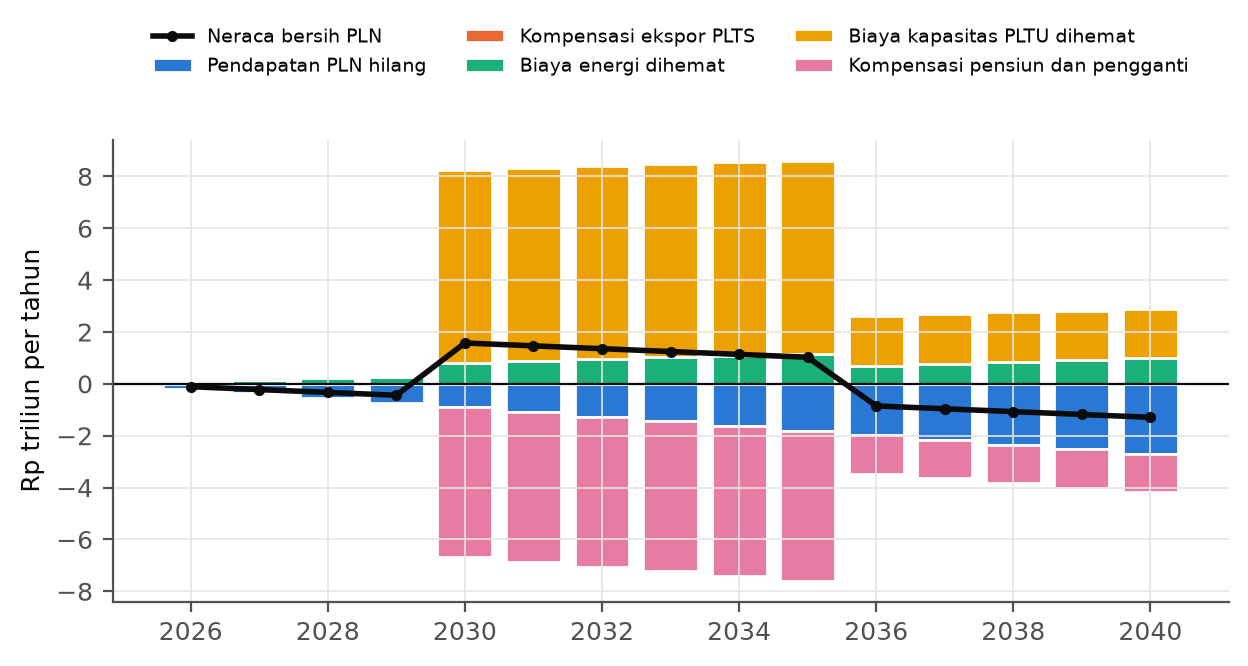
\includegraphics[width=\textwidth]{neraca_seimbang}
\caption{Komponen neraca PLN per tahun pada Paket seimbang}
\label{fig:seimbang}
\sumber{simulasi PowerShift}
\end{figure}

Gambar~\ref{fig:seimbang} menjelaskan sumber keseimbangan itu. Selama 2030-2035, PLN menghemat pembayaran kapasitas IPP sekitar Rp7 triliun per tahun. Penghematan ini mengimbangi porsi kompensasi dan biaya 2.580 MW pembangkit pengganti. Setelah 2036, tiga dari empat PLTU memang sudah pensiun di baseline, sehingga selisihnya mengecil. Gambar~\ref{fig:rm} menunjukkan bahwa tanpa pembangkit pengganti, reserve margin akan turun ke 25,9\%. Karena itu, biaya pengganti dihitung sebagai bagian dari paket.

\begin{figure}[H]
\centering
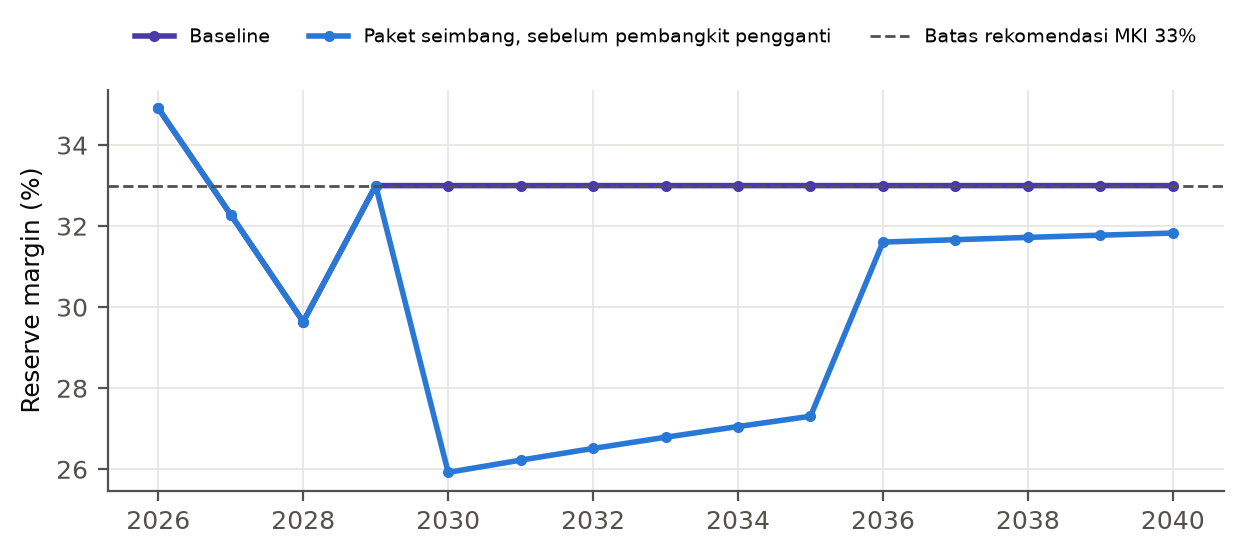
\includegraphics[width=\textwidth]{reserve_margin}
\caption{Reserve margin baseline dan Paket seimbang sebelum pembangkit pengganti}
\label{fig:rm}
\sumber{simulasi PowerShift berdasarkan \textcite{B-MATAHARI-2024} dan \textcite{B-PETROMINDO-RESERVE}}
\end{figure}

Pilihan PLTU sangat menentukan. Pensiun PLTU milik PLN, misalnya Pelabuhan Ratu, justru membebani PLN karena tidak ada pembayaran kapasitas yang dapat dihemat, sementara nilai buku dan pembangkit pengganti tetap harus ditanggung. Sebaliknya, Cirebon-1 memberi manfaat kesehatan terbesar per MW karena lokasinya.

\subsection{Biaya dan Pelaksana}

Biaya pengembangan PowerShift hanya waktu kerja tim. Biaya operasinya nol karena berupa situs statis dengan hosting gratis dan data terbuka. Pelaksana yang diusulkan:
\begin{itemize}
  \item \textbf{Ditjen Ketenagalistrikan ESDM dan tim kerja gabungan Pasal 14 Permen ESDM 10/2025}: pengguna utama untuk menilai usulan pensiun dini.
  \item \textbf{PLN}: mengganti parameter kontrak IPP dengan data sebenarnya saat menyusun kajian enam bulan.
  \item \textbf{Dinas ESDM Jawa Barat}: menyorot Cirebon-1 dan kontribusi PLTS atap provinsi.
  \item \textbf{Kampus atau lembaga riset energi}: memelihara data dan model sebagai barang publik.
\end{itemize}

\subsection{Kebijakan Pendukung}

PowerShift memanfaatkan kerangka yang sudah ada. Permen ESDM 10/2025 mewajibkan kajian teknis, hukum, komersial, dan keuangan serta membuka penggunaan kajian lembaga independen sebagai rujukan \parencite{B-CNN-20250422}. Kuota PLTS atap 5.746 MW untuk 2024-2028 \parencite{B-PVMAG-QUOTA} dan rencana 33,5 GW pembangkit baru di Jamali, termasuk 10,9 GW surya \parencite{B-LISTRIKID-RUPTL-JAMALI}, memberi ruang untuk menguji paket. Usulan IESR untuk mengalihkan subsidi 450/900 VA ke PLTS atap \parencite{B-KABARBURSA-SUBSIDI} juga dapat diuji langsung di alat.

\subsection{Risiko}

\begin{figure}[H]
\centering
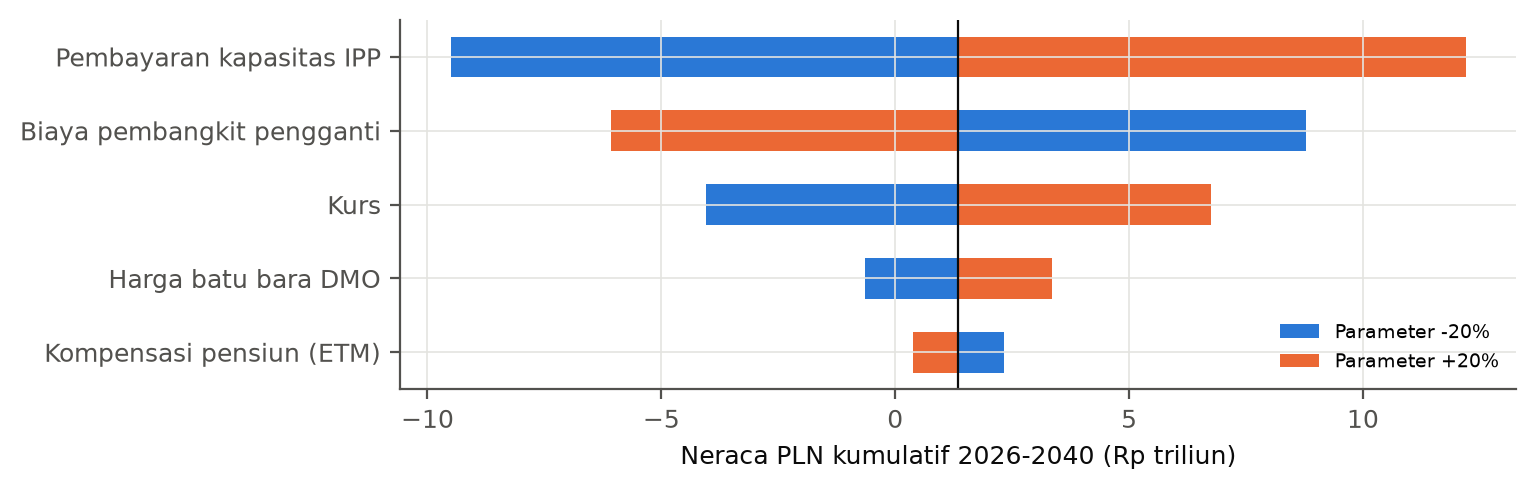
\includegraphics[width=\textwidth]{tornado_seimbang}
\caption{Sensitivitas neraca PLN Paket seimbang terhadap perubahan parameter $\pm$20\%}
\label{fig:tornado}
\sumber{simulasi PowerShift}
\end{figure}

Risiko terbesar adalah ketidakpastian data kontrak IPP. Gambar~\ref{fig:tornado} menunjukkan bahwa neraca Paket seimbang paling peka terhadap besaran pembayaran kapasitas IPP dan biaya pembangkit pengganti. Perubahan 20\% dapat menggeser hasil sekitar Rp7-11 triliun. Risiko lain adalah klaim kompensasi yang jauh lebih tinggi. Dengan klaim PLN untuk Cirebon-1 (sekitar Rp18 miliar per MW per tahun dipercepat), neraca PLN memburuk tajam. Mitigasinya, semua asumsi ditampilkan terbuka dan dapat diubah, sehingga perbedaan angka antara PLN, ADB, dan pemerintah dapat diperdebatkan secara transparan. Model ini juga tidak menggantikan simulasi jaringan per jam, sehingga hasilnya bersifat indikatif.

\subsection{Ukuran Keberhasilan}

\begin{itemize}
  \item Teknis: halaman terbuka di bawah 3 detik, perhitungan ulang instan, hitung tangan cocok dengan aplikasi (sudah tercapai).
  \item Isi: minimal 70\% parameter kunci berstatus terverifikasi. Saat ini 18 dari 42 parameter terverifikasi, 21 asumsi terdokumentasi, dan 3 masih perlu dicek ke sumber asli.
  \item Pemakaian: PowerShift dipakai dalam minimal satu diskusi kebijakan atau kajian pensiun dini, dan skenario dibagikan antarpemangku kepentingan.
\end{itemize}

\section{Rekomendasi}
\label{sec:rekomendasi}

\subsection{Langkah Konkret}

\begin{enumerate}
  \item \textbf{Prioritaskan IPP tua dengan dampak kesehatan tinggi.} Pensiun dini paling layak secara keuangan untuk PLTU IPP yang pembayaran kapasitasnya masih berjalan. Prioritaskan unit yang juga memiliki biaya kesehatan per kWh tinggi, seperti Cirebon-1.
  \item \textbf{Pastikan kompensasi didanai dari luar neraca PLN.} H2 hanya berlaku bila sebagian besar kompensasi berasal dari ETM/JETP atau dana iklim. Tanpa itu, pensiun dini memindahkan beban ke tarif dan APBN.
  \item \textbf{Hitung pembangkit pengganti sejak awal.} Jendela oversupply Jawa-Bali praktis menutup pada 2027-2028. Setiap usulan pensiun dini setelahnya perlu memasukkan biaya pengganti bersih, misalnya PLTS skala besar dengan baterai.
  \item \textbf{Dorong PLTS atap lewat jalur yang tidak memukul pendapatan PLN.} Jalur yang paling seimbang adalah gedung pemerintah, karena tagihan yang dihemat kembali ke APBN. Mengembalikan net metering secara luas membutuhkan mekanisme kompensasi pendapatan PLN, misalnya dari dana iklim yang dihitung dari nilai kesehatan.
  \item \textbf{Gunakan alat terbuka dalam kajian Permen ESDM 10/2025.} Kajian enam bulan PLN dan evaluasi tim kerja gabungan sebaiknya memakai asumsi yang dapat diperiksa publik, misalnya lewat PowerShift.
\end{enumerate}

\subsection{Peran Aktor}

\begin{table}[H]
\centering
\caption{Pembagian peran aktor}
\label{tab:aktor}
\small
\begin{tabularx}{\textwidth}{p{0.24\textwidth} X}
\toprule
Aktor & Tindakan \\
\midrule
Kementerian ESDM & Menetapkan daftar kandidat pensiun dini berbasis kriteria Pasal 11 dan biaya kesehatan, memakai alat terbuka dalam evaluasi tim kerja gabungan \\
PLN & Menyediakan data pembayaran kapasitas dan akhir PPA untuk kajian, menghitung kebutuhan pembangkit pengganti \\
Kementerian Keuangan & Menyusun skema kompensasi dari dana luar dan menghitung penghematan subsidi serta tagihan pemerintah \\
Mitra ETM/JETP dan ADB & Mengalihkan dana Cirebon-1 ke paket IPP tua dengan dampak kesehatan tinggi \\
Pemerintah daerah & Memasang PLTS atap di gedung pemerintah dan menyiapkan program alih keterampilan pekerja PLTU \\
Akademisi dan masyarakat sipil & Memelihara data dan model PowerShift, menyosialisasikan hasil kepada publik \\
\bottomrule
\end{tabularx}
\end{table}

Secara keseluruhan, transisi PLTS atap dan pensiun dini PLTU macet karena manfaatnya dirasakan masyarakat (kesehatan, tagihan) sementara biayanya jatuh ke PLN dan APBN. Paket yang memilih PLTU dengan tepat, mendanai kompensasi dari luar, dan memasang PLTS atap lewat jalur pemerintah dapat menyeimbangkan kedua sisi itu.

\section{Tabel Kontribusi}
\label{sec:kontribusi}

Kelompok 17 terdiri atas Tim Laporan, Tim PPT, dan Tim Presentasi. Rincian kontribusi mengikuti pembagian kerja pada laporan kelompok. Anggota yang rinciannya tidak tercatat ditulis sesuai peran timnya.

{\small
\begin{longtable}{p{0.04\textwidth} p{0.27\textwidth} p{0.11\textwidth} p{0.1\textwidth} p{0.34\textwidth}}
\toprule
No & Nama & NIM & Tim & Kontribusi \\
\midrule
\endhead
1 & Lidya Savarani Tarigan & 15024071 & Laporan & Menyusun subbab 1.1 sampai 1.5 laporan kelompok (latar belakang, rumusan masalah, tujuan, ruang lingkup, manfaat) dan membagi serta memantau tugas subkelompok laporan \\
2 & Pande I Made Niko Mevano W P & 10623042 & Laporan & Penyusunan laporan kelompok \\
3 & Haidar Islama Muhammad Firdaus & 15524057 & Laporan & Menyusun subbab 2.3 analisis dampak PLTU terhadap sosial dan masyarakat beserta referensinya \\
4 & Nayma Feby Nur Safitri & 10524057 & Laporan & Penyusunan laporan kelompok \\
5 & Alya Gita Khairani & 15325093 & Laporan & Penyusunan laporan kelompok \\
6 & Isnaya Zalfa Kamila & 13224028 & Laporan & Penyusunan laporan kelompok \\
7 & Kayla Olivia Putri & 18124013 & Laporan & Penyusunan laporan kelompok \\
8 & Bram Sebastian Pangaribuan & 18224076 & Laporan & Menginisiasi format laporan ilmiah kelompok dan melakukan proofread dokumen laporan \\
9 & Muhammad Rafi Hikaru Rahman & 15325021 & Laporan & Menyusun subbab 4.1 kebaruan inovasi: risiko ekonomi, kapasitas fiskal, aset terbengkalai, dan perbandingan dengan kajian terdahulu \\
10 & Ananda Ghibran Fadlilah & 13123086 & Laporan & Penyusunan laporan kelompok \\
11 & Muhammad Azhar Shiddiq & 13123129 & Laporan & Penyusunan laporan kelompok \\
12 & Dimas Rayhan & 12023096 & Laporan & Menyusun subbab 3.4 matriks perbandingan opsi, 5.1 estimasi biaya, dan 5.4 indikator keberhasilan, serta daftar isi, daftar tabel, dan daftar pustaka \\
13 & Azzahra Rizqi Saffa & 10124084 & Laporan & Menyusun subbab 4.3 kontekstualisasi dan uji kesesuaian Indonesia \\
14 & Alzena Atha Audya & 15024052 & PPT & Penyusunan materi presentasi \\
15 & Magdalena Conny H.C.L.T & 13424036 & PPT & Penyusunan materi presentasi \\
16 & Danica Giovanni & 10524012 & PPT & Penyusunan materi presentasi \\
17 & Angga Setiawan & 15124066 & PPT & Penyusunan materi presentasi \\
18 & Franzeska Jessica Mattea & 12225128 & PPT & Penyusunan materi presentasi \\
19 & Elja Manuella Joesta Damanik & 15325014 & PPT & Menyusun slide presentasi bagian latar belakang, tujuan, rumusan masalah, dan manfaat \\
20 & Muhamad Nazih Najmudin & 13523144 & PPT & Menyusun slide presentasi bagian opsi adaptasi, mengembangkan platform PowerShift, serta menyusun laporan dan dokumen kajian PowerShift \\
21 & Raynee Soe Putra & 18023017 & Presentasi & Menyusun rencana pengerjaan dan gagasan awal, menyiapkan naskah, dan menjadi juru bicara presentasi \\
22 & Jessica Aulia Cahyana & 15124027 & Presentasi & Persiapan dan penyampaian presentasi \\
23 & Fahri Masis Nurhidayat & 12324059 & Presentasi & Persiapan dan penyampaian presentasi \\
24 & Qabil Radhiqa Handoyo & 15124032 & Presentasi & Persiapan dan penyampaian presentasi \\
\bottomrule
\end{longtable}

}


\clearpage
\printbibliography[title={Daftar Pustaka}]

\clearpage
\appendix
\section{Hitung Tangan Paket Cirebon-1}
\label{app:hitung}

Hitung tangan disusun independen dari kode aplikasi untuk preset Paket Cirebon-1: nilai ekspor 65\%, kuota 1.500 MW per tahun, gedung pemerintah 100 MW per tahun, 5\% subsidi dialihkan, Cirebon-1 pensiun 2035, dan 25\% kompensasi ditanggung PLN. Selisih dengan hasil aplikasi di bawah 0,01\% untuk seluruh komponen.

\begin{table}[H]
\centering
\caption{Hitung tangan neraca PLN Paket Cirebon-1 terhadap baseline}
\small
\begin{tabular}{lrrr}
\toprule
Komponen (Rp T, kecuali disebut) & 2030 & 2035 & 2040 \\
\midrule
Kapasitas PLTS atap (MWp) & 5.937 & 12.525 & 19.112 \\
Pendapatan PLN hilang & -4,80 & -10,54 & -16,29 \\
Kompensasi ekspor PLTS & -2,87 & -6,44 & -10,01 \\
Biaya energi dihemat & 3,03 & 6,75 & 10,55 \\
Pembayaran kapasitas dihemat & 0,00 & 1,91 & 1,91 \\
Porsi PLN kompensasi pensiun & 0,00 & -0,17 & -0,17 \\
Pembangkit pengganti & 0,00 & -1,31 & -1,31 \\
Neraca PLN & -4,64 & -9,80 & -15,32 \\
\bottomrule
\end{tabular}

\end{table}

Langkah perhitungan:
\begin{enumerate}
  \item PVOUT rata-rata tertimbang penjualan listrik PLN per provinsi: 1.423,5 kWh/kWp per tahun.
  \item Balik modal rumah tangga non subsidi tanpa ekspor: Rp15 juta / (1.423,5 $\times$ 1.444,70 $\times$ 0,4) = 18,2 tahun. Dengan ekspor 65\%: 9,2 tahun.
  \item Tambahan pasar = tren $\times$ porsi segmen $\times$ exp($-$0,3 $\times$ 9,2) / exp($-$0,3 $\times$ 18,2), naik bertahap selama 4 tahun dan dibatasi kuota.
  \item Biaya marjinal armada PLTU: Rp494 per kWh dari harga DMO US\$70 per ton dan heat rate GEM.
  \item Cirebon-1 pada 2035: pembayaran kapasitas 660 MW $\times$ US\$175/kW $\times$ Rp16.500 = Rp1,91 triliun. Porsi PLN kompensasi 25\% $\times$ Rp1,045 miliar $\times$ 660 MW = Rp0,17 triliun. Pembangkit pengganti 660 MW $\times$ US\$120/kW $\times$ Rp16.500 = Rp1,31 triliun.
\end{enumerate}

\section{Tabel Asumsi}
\label{app:asumsi}

Status ``terverifikasi'' berarti angka dicocokkan dengan dokumen sumber. Kode sumber mengacu pada daftar pustaka (lihat juga halaman Sumber di aplikasi).

{\small
\begin{longtable}{p{0.33\textwidth} p{0.2\textwidth} p{0.26\textwidth} p{0.11\textwidth}}
\toprule
Parameter & Nilai & Sumber & Status \\
\midrule
\endhead
Tahun dasar & 2025 tahun & \texttt{-\allowbreak{}} & asumsi \\
Beban puncak tertinggi Jawa-Madura-Bali & 28.077 MW & \texttt{B-\allowbreak{}MATAHARI-\allowbreak{}2024} & terverifikasi \\
Reserve margin Jawa-Madura-Bali 2025 & 0,375 fraksi & \texttt{B-\allowbreak{}PETROMINDO-\allowbreak{}RESERVE} & terverifikasi \\
Pertumbuhan beban dan penjualan & 0,0445 per tahun & \texttt{B-\allowbreak{}PETROMINDO-\allowbreak{}RESERVE} & terverifikasi \\
Tambahan daya mampu 2026-2028 & 1.000 MW/tahun & \texttt{B-\allowbreak{}PETROMINDO-\allowbreak{}RESERVE} & asumsi \\
Batas bawah reserve margin yang direkomendasikan & 0,33 fraksi & \texttt{B-\allowbreak{}PETROMINDO-\allowbreak{}RESERVE} & terverifikasi \\
Penjualan listrik PLN 2025 & 317,69 TWh & \texttt{B-\allowbreak{}CNBC-\allowbreak{}SALES-\allowbreak{}2025} & terverifikasi \\
Porsi penjualan Jawa-Bali & 0,695 fraksi & \texttt{D-\allowbreak{}PLN-\allowbreak{}STAT-\allowbreak{}2025} & terverifikasi \\
Biaya pokok penyediaan 2026 & 1.874 Rp/kWh & \texttt{B-\allowbreak{}KONTAN-\allowbreak{}SUBSIDI-\allowbreak{}2026} & terverifikasi \\
Kurs & 16.500 Rp/US\$ & \texttt{B-\allowbreak{}KONTAN-\allowbreak{}SUBSIDI-\allowbreak{}2026} & terverifikasi \\
Tingkat diskonto NPV & 0,08 per tahun & \texttt{assumption} & asumsi \\
Porsi kerugian PLN yang ditutup APBN & 1 fraksi & \texttt{assumption} & asumsi \\
Mulai tahun PLN menambah pembangkit untuk menjaga target cadangan & 2029 tahun & \texttt{B-\allowbreak{}LISTRIKID-\allowbreak{}RUPTL-\allowbreak{}JAMALI} & asumsi \\
Harga batu bara DMO untuk PLN & 70 US\$/ton & \texttt{B-\allowbreak{}KONTAN-\allowbreak{}DMO-\allowbreak{}2026} & terverifikasi \\
Kalori acuan harga DMO & 6.322 kcal/kg & \texttt{B-\allowbreak{}KONTAN-\allowbreak{}DMO-\allowbreak{}2026} & perlu cek \\
Biaya variabel non bahan bakar PLTU & 50 Rp/kWh & \texttt{assumption} & asumsi \\
Pembayaran kapasitas IPP (komponen A) & 175 US\$/kW/tahun & \texttt{P-\allowbreak{}IEEFA-\allowbreak{}2017} & asumsi \\
Biaya tetap O\&M PLTU milik PLN & 40 US\$/kW/tahun & \texttt{assumption} & asumsi \\
Nilai buku PLTU milik PLN tahun 2022 & 762.000 US\$/MW & \texttt{B-\allowbreak{}PELABUHANRATU-\allowbreak{}VALUASI} & perlu cek \\
Kompensasi pensiun dini, estimasi skema ETM & 1,04 miliar Rp/MW/tahun dipercepat & \texttt{B-\allowbreak{}REUTERS-\allowbreak{}CIREBON-\allowbreak{}2022} & terverifikasi \\
Kompensasi pensiun dini, klaim PLN & 18,18 miliar Rp/MW/tahun dipercepat & \texttt{B-\allowbreak{}PETROMINDO-\allowbreak{}CIREBON-\allowbreak{}BATAL} & terverifikasi \\
Pekerja langsung per MW & 0,4545 orang/MW & \texttt{B-\allowbreak{}ECOBUSINESS-\allowbreak{}CIREBON} & terverifikasi \\
Biaya kapasitas pembangkit pengganti & 120 US\$/kW/tahun & \texttt{assumption} & asumsi \\
Kematian dini rata-rata armada PLTU & 258,6 kematian/GW/tahun & \texttt{P-\allowbreak{}CREA-\allowbreak{}IESR-\allowbreak{}2023} & terverifikasi \\
Biaya kesehatan per kematian & 704.762 US\$/kematian & \texttt{P-\allowbreak{}CREA-\allowbreak{}IESR-\allowbreak{}2023} & terverifikasi \\
PLTS atap terpasang nasional Juli 2025 & 538 MWp & \texttt{B-\allowbreak{}KONTAN-\allowbreak{}ROOFTOP-\allowbreak{}2025} & terverifikasi \\
Porsi PLTS atap di Jawa-Bali & 0,8 fraksi & \texttt{assumption} & asumsi \\
Tambahan PLTS atap Jawa-Bali dengan aturan sekarang & 240 MWp/tahun & \texttt{B-\allowbreak{}KONTAN-\allowbreak{}ROOFTOP-\allowbreak{}2025} & asumsi \\
Kuota PLTS atap Jawa-Bali per tahun & 800 MW/tahun & \texttt{B-\allowbreak{}PVMAG-\allowbreak{}QUOTA} & asumsi \\
Koefisien kurva pangsa pasar vs balik modal & 0,3 1/tahun & \texttt{P-\allowbreak{}NREL-\allowbreak{}SOLARDS} & perlu cek \\
Umur PLTS atap & 25 tahun & \texttt{assumption} & asumsi \\
Lapangan kerja PLTS atap & 24,72 job-year/MW & \texttt{P-\allowbreak{}CEEW-\allowbreak{}2017} & terverifikasi \\
Keluaran puncak AC per kWp & 0,75 fraksi & \texttt{assumption} & asumsi \\
PLTS atap: Rumah tangga non subsidi & Rp15 jt/kWp, pakai sendiri 40\%, tarif Rp1.444,70 & \texttt{B-\allowbreak{}KOMPASTV-\allowbreak{}TARIF-\allowbreak{}2026} & asumsi \\
PLTS atap: Bisnis & Rp13 jt/kWp, pakai sendiri 80\%, tarif Rp1.224,83 & \texttt{D-\allowbreak{}PLN-\allowbreak{}STAT-\allowbreak{}2025} & asumsi \\
PLTS atap: Industri & Rp11 jt/kWp, pakai sendiri 90\%, tarif Rp1.085,39 & \texttt{D-\allowbreak{}PLN-\allowbreak{}STAT-\allowbreak{}2025} & asumsi \\
PLTS atap: Gedung pemerintah & Rp13 jt/kWp, pakai sendiri 80\%, tarif Rp1.583,12 & \texttt{D-\allowbreak{}PLN-\allowbreak{}STAT-\allowbreak{}2025} & asumsi \\
PLTS atap: Program rumah tangga subsidi & Rp12 jt/kWp, pakai sendiri 50\%, tarif Rp605,00 & \texttt{B-\allowbreak{}KOMPASTV-\allowbreak{}TARIF-\allowbreak{}2026} & asumsi \\
Lama respons pasar PLTS atap terhadap perubahan aturan & 4 tahun & \texttt{assumption} & asumsi \\
Subsidi listrik 2026 & 101.170 miliar Rp/tahun & \texttt{B-\allowbreak{}KONTAN-\allowbreak{}SUBSIDI-\allowbreak{}2026} & terverifikasi \\
Pelanggan subsidi 2026 & 44.880.000 pelanggan & \texttt{B-\allowbreak{}KONTAN-\allowbreak{}SUBSIDI-\allowbreak{}2026} & terverifikasi \\
Porsi subsidi di Jawa-Bali & 0,61 fraksi & \texttt{D-\allowbreak{}PLN-\allowbreak{}STAT-\allowbreak{}2025} & asumsi \\
\bottomrule
\end{longtable}

}

\section{Daftar Unit PLTU}
\label{app:data}

Unit PLTU operasi terhubung jaringan PLN di Jawa-Bali \parencite{D-GEM-GCPT}. Tahun pensiun baseline memakai rencana pensiun GEM jika ada, akhir PPA 30 tahun untuk IPP, atau umur desain 40 tahun untuk PLTU milik PLN.

{\small
\begin{longtable}{p{0.22\textwidth} p{0.15\textwidth} r r l r r}
\toprule
PLTU & Unit & MW & Mulai & Tipe & Pensiun baseline & tCO$_2$/MWh \\
\midrule
\endhead
Adipala & Unit 1 & 660 & 2015 & PLN & 2055 & 0,94 \\
Batang (Central Java Power) & Unit 1 & 950 & 2022 & IPP & 2052 & 0,84 \\
Batang (Central Java Power) & Unit 2 & 950 & 2022 & IPP & 2052 & 0,84 \\
Celukan Bawang & Unit 1 & 142 & 2015 & IPP & 2045 & 1,15 \\
Celukan Bawang & Unit 2 & 142 & 2015 & IPP & 2045 & 1,15 \\
Celukan Bawang & Unit 3 & 142 & 2015 & IPP & 2045 & 1,15 \\
Cilacap Sumber & Phase I Unit 1 & 300 & 2006 & IPP & 2036 & 1,15 \\
Cilacap Sumber & Phase I Unit 2 & 300 & 2006 & IPP & 2036 & 1,15 \\
Cilacap Sumber & Phase II Unit 3 & 660 & 2016 & IPP & 2046 & 0,94 \\
Cilacap Sumber & Phase III Unit 4 & 1.000 & 2019 & IPP & 2049 & 0,84 \\
Cirebon & Unit 1 & 660 & 2012 & IPP & 2042 & 0,94 \\
Cirebon & Unit 2 & 924 & 2023 & IPP & 2053 & 0,84 \\
Indramayu & Unit 1 & 330 & 2010 & PLN & 2050 & 1,06 \\
Indramayu & Unit 2 & 330 & 2011 & PLN & 2051 & 1,06 \\
Indramayu & Unit 3 & 330 & 2011 & PLN & 2051 & 1,06 \\
Jawa-7 & Unit 1 & 991 & 2019 & IPP & 2049 & 0,84 \\
Jawa-7 & Unit 2 & 991 & 2020 & IPP & 2050 & 0,84 \\
Labuan & Unit 1 & 300 & 2009 & PLN & 2049 & 1,06 \\
Labuan & Unit 2 & 300 & 2010 & PLN & 2050 & 1,06 \\
Lontar & Unit 1 & 315 & 2011 & PLN & 2051 & 1,06 \\
Lontar & Unit 2 & 315 & 2012 & PLN & 2052 & 1,06 \\
Lontar & Unit 3 & 315 & 2012 & PLN & 2052 & 1,06 \\
Lontar & Unit 4 & 315 & 2024 & PLN & 2064 & 0,92 \\
Pacitan & Unit 1 & 315 & 2011 & PLN & 2051 & 1,06 \\
Pacitan & Unit 2 & 315 & 2011 & PLN & 2051 & 1,06 \\
Paiton & Unit 1 & 400 & 1994 & PLN & 2030 & 1,19 \\
Paiton & Unit 2 & 400 & 1993 & PLN & 2033 & 1,19 \\
Paiton Baru & Unit 09 & 660 & 2012 & PLN & 2052 & 0,97 \\
Paiton-1 & Unit 7 & 615 & 1999 & IPP & 2029 & 1,06 \\
Paiton-1 & Unit 8 & 615 & 1999 & IPP & 2029 & 1,06 \\
Paiton-2 & Unit 1 & 660 & 2000 & IPP & 2030 & 1,06 \\
Paiton-2 & Unit 2 & 660 & 2000 & IPP & 2030 & 1,06 \\
Paiton-3 & Unit 1 & 815 & 2012 & IPP & 2042 & 0,94 \\
Pelabuhan Ratu & Unit 1 & 350 & 2013 & PLN & 2045 & 1,06 \\
Pelabuhan Ratu & Unit 2 & 350 & 2013 & PLN & 2045 & 1,06 \\
Pelabuhan Ratu & Unit 3 & 350 & 2013 & PLN & 2045 & 1,06 \\
Rembang & Unit 1 & 315 & 2011 & PLN & 2051 & 1,06 \\
Rembang & Unit 2 & 315 & 2011 & PLN & 2051 & 1,06 \\
Serang & Unit 1 & 660 & 2017 & IPP & 2047 & 0,85 \\
Suralaya & Phase I Unit 1 & 400 & 1984 & PLN & 2030 & 1,19 \\
Suralaya & Phase I Unit 2 & 400 & 1985 & PLN & 2030 & 1,19 \\
Suralaya & Phase I Unit 3 & 400 & 1988 & PLN & 2030 & 1,19 \\
Suralaya & Phase I Unit 4 & 400 & 1989 & PLN & 2030 & 1,19 \\
Suralaya & Phase II Unit 1 & 600 & 1996 & PLN & 2036 & 1,10 \\
Suralaya & Phase II Unit 2 & 600 & 1997 & PLN & 2037 & 1,06 \\
Suralaya & Phase II Unit 3 & 600 & 1997 & PLN & 2037 & 1,06 \\
Suralaya & Unit 08 & 625 & 2011 & PLN & 2051 & 0,97 \\
Suralaya & Unit 09 & 1.000 & 2025 & IPP & 2055 & 0,84 \\
Suralaya & Unit 10 & 1.000 & 2025 & IPP & 2055 & 0,84 \\
Tanjung Awar-Awar & Unit 1 & 350 & 2012 & PLN & 2052 & 1,06 \\
Tanjung Awar-Awar & Unit 2 & 350 & 2013 & PLN & 2053 & 1,06 \\
Tanjung Jati B & Unit 1 & 660 & 2006 & IPP & 2036 & 1,04 \\
Tanjung Jati B & Unit 2 & 660 & 2006 & IPP & 2036 & 1,04 \\
Tanjung Jati B & Unit 3 & 660 & 2011 & IPP & 2041 & 0,95 \\
Tanjung Jati B & Unit 4 & 660 & 2012 & IPP & 2042 & 0,95 \\
Tanjung Jati B & Unit 5 & 1.000 & 2022 & IPP & 2047 & 0,84 \\
Tanjung Jati B & Unit 6 & 1.000 & 2022 & IPP & 2047 & 0,84 \\
\bottomrule
\end{longtable}

}


\end{document}
